\documentclass{exam}
\usepackage{main}

\title{Evaluation de cours}
\date{25 Mars 2024}
\author{Quentin Canu}

\begin{document}
\maketitle
\thispagestyle{empty}

\paragraph*{Version 1}
\begin{questions}
\question Remettre dans l'ordre la démonstration de la croissance de la fonction $f : x \mapsto x^2$ sur $\left[0;+\infty\right[$.
\begin{parts}
\part On conclut que $f$ est croissante sur $\left[0;+\infty\right[$     
\part Puisque $x \geq 0$, $y \geq 0$ et $x \leq y$, on en déduit que $0 \leq y^2 - x^2$.
\part On veut montrer que $x^2 \leq y^2$, ou de manière équivalente que $0 \leq y^2 - x^2$.
\part Soient $x$ et $y$ positifs. On suppose $x \leq y$.
\part Or, $y^2 - x^2 = (y-x)(y+x)$. 
\end{parts}
\vspace*{1cm}
\question Soit $f$ une fonction dont la courbe représentative $\mathcal{C}_f$ est donnée ci-après. Tracer le tableau de variations de $f$.
\begin{center}
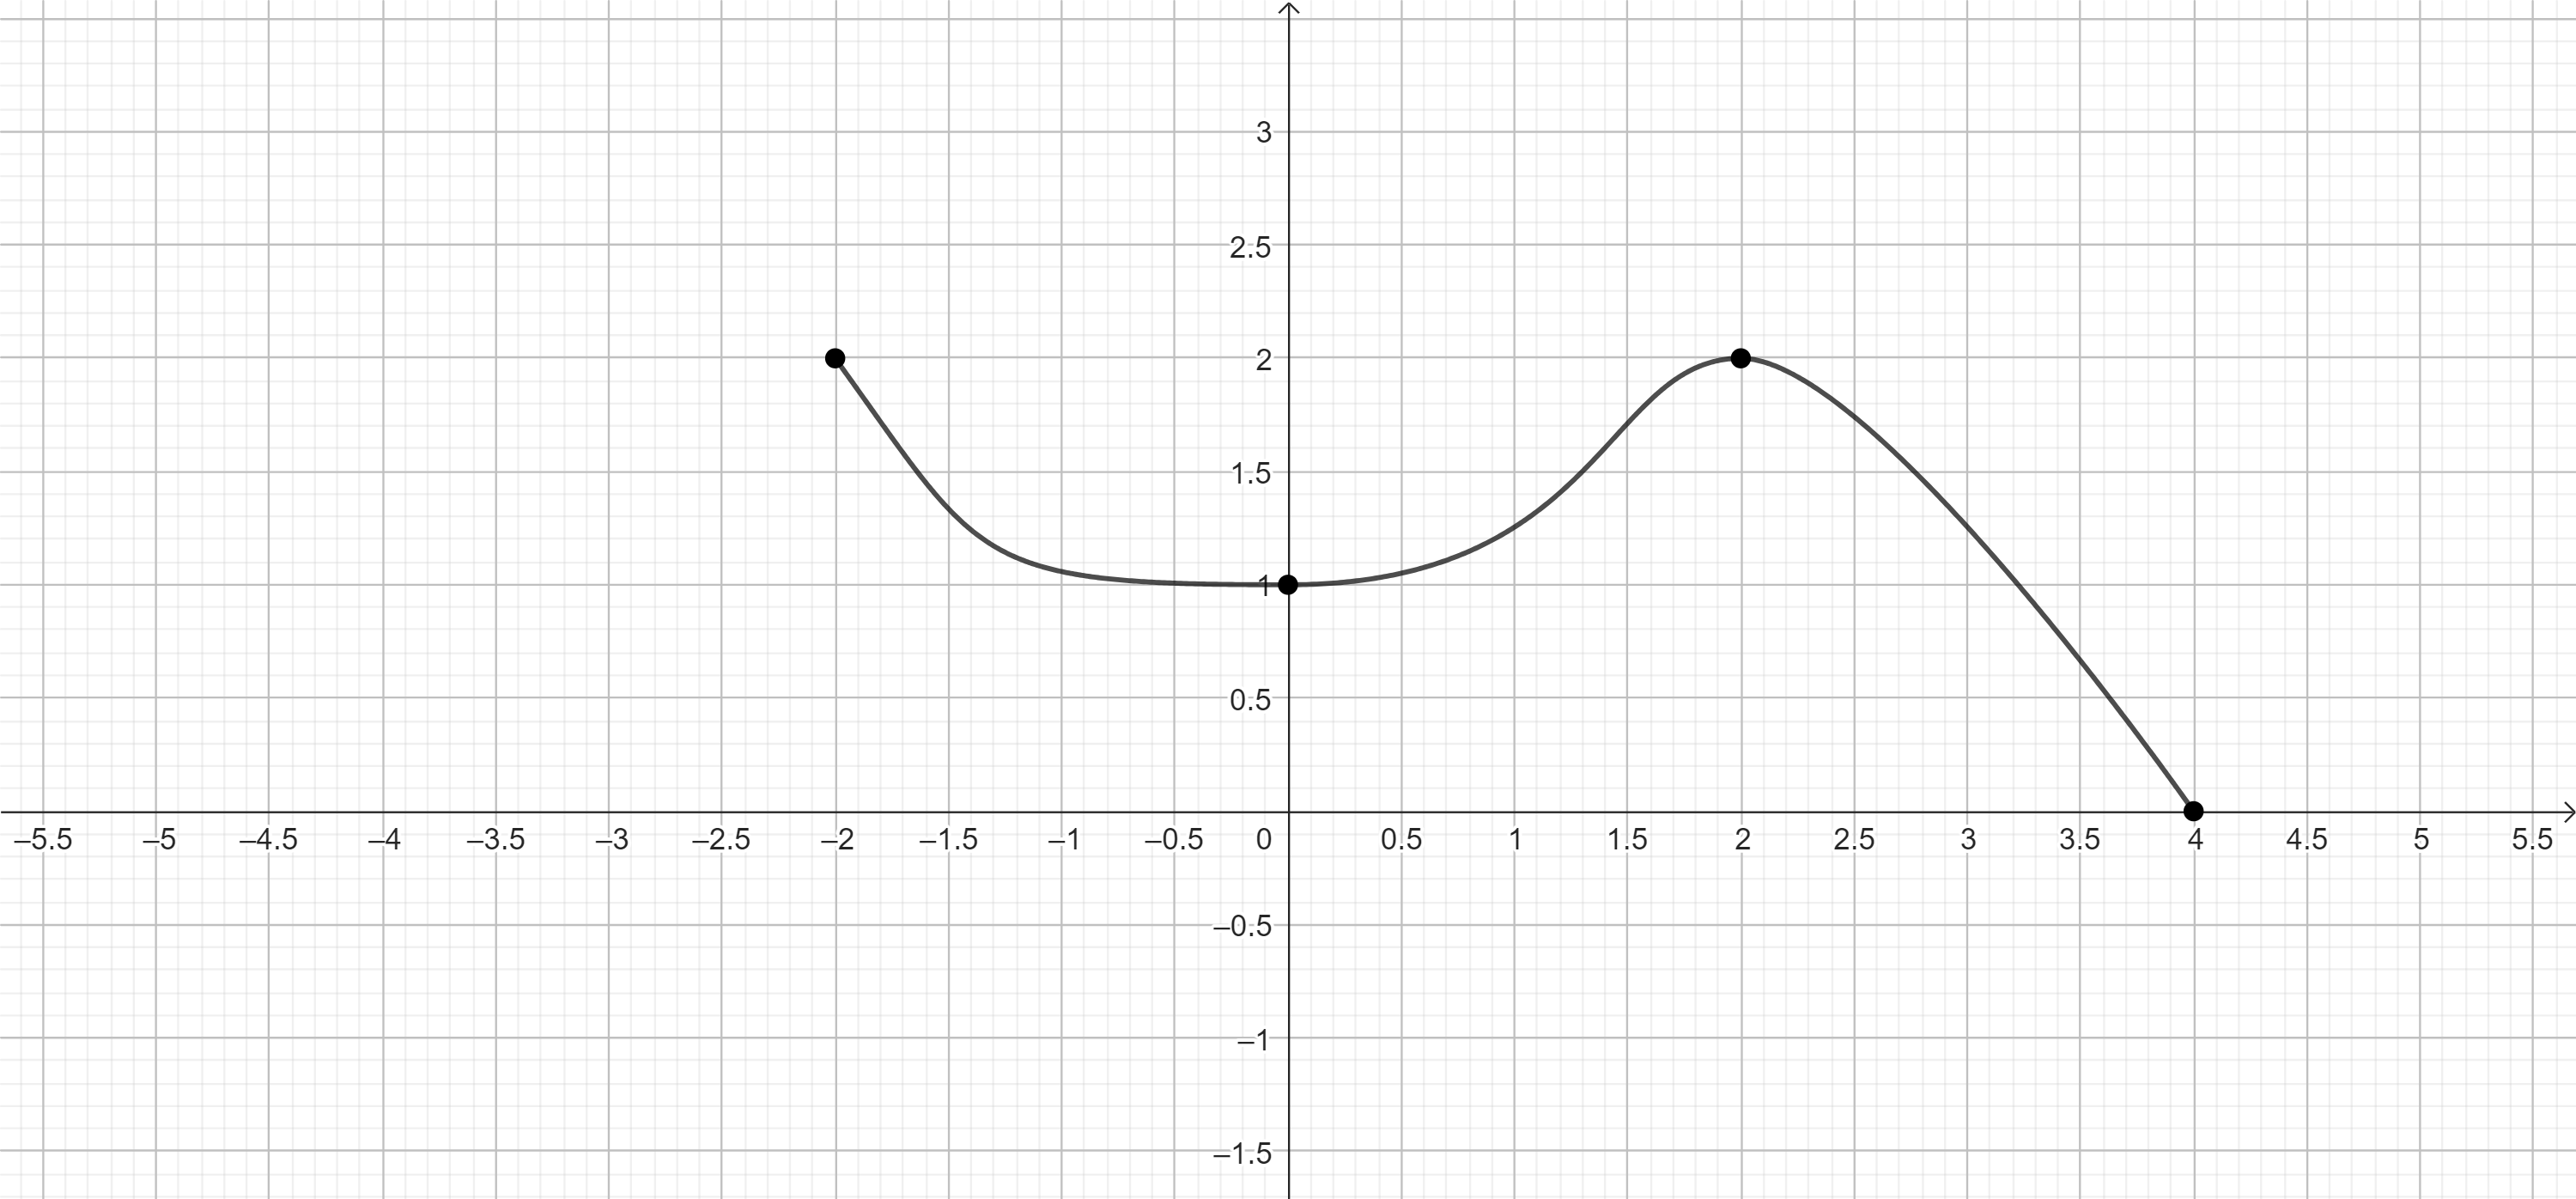
\includegraphics[scale=1.5]{Fonction1.png}
\end{center}
\end{questions}

\newpage

\maketitle
\thispagestyle{empty}
\paragraph*{Version 2}
\begin{questions}
\question Remettre dans l'ordre la démonstration de la croissance de la fonction $f : x \mapsto \sqrt{x}$ sur $\left[0;+\infty\right[$.
\begin{parts}
\part Soient $x$ et $y$ positifs. On suppose $x \leq y$.
\part Or, $\sqrt{y} - \sqrt{x} = \dfrac{y-x}{\sqrt{y}+\sqrt{x}}$. 
\part Puisque $\sqrt{x} \geq 0$, $\sqrt{y} \geq 0$ et $x \leq y$, on en déduit que $0 \leq \sqrt{y} - \sqrt{x}$.
\part On conclut que $f$ est croissante sur $\left[0;+\infty\right[$     
\part On veut montrer que $\sqrt{x} \leq \sqrt{y}$, ou de manière équivalente que $0 \leq \sqrt{y} - \sqrt{x}$.
\end{parts}
\vspace*{1cm}
\question Soit $f$ une fonction dont la courbe représentative $\mathcal{C}_f$ est donnée ci-après. Tracer le tableau de variations de $f$.
\begin{center}
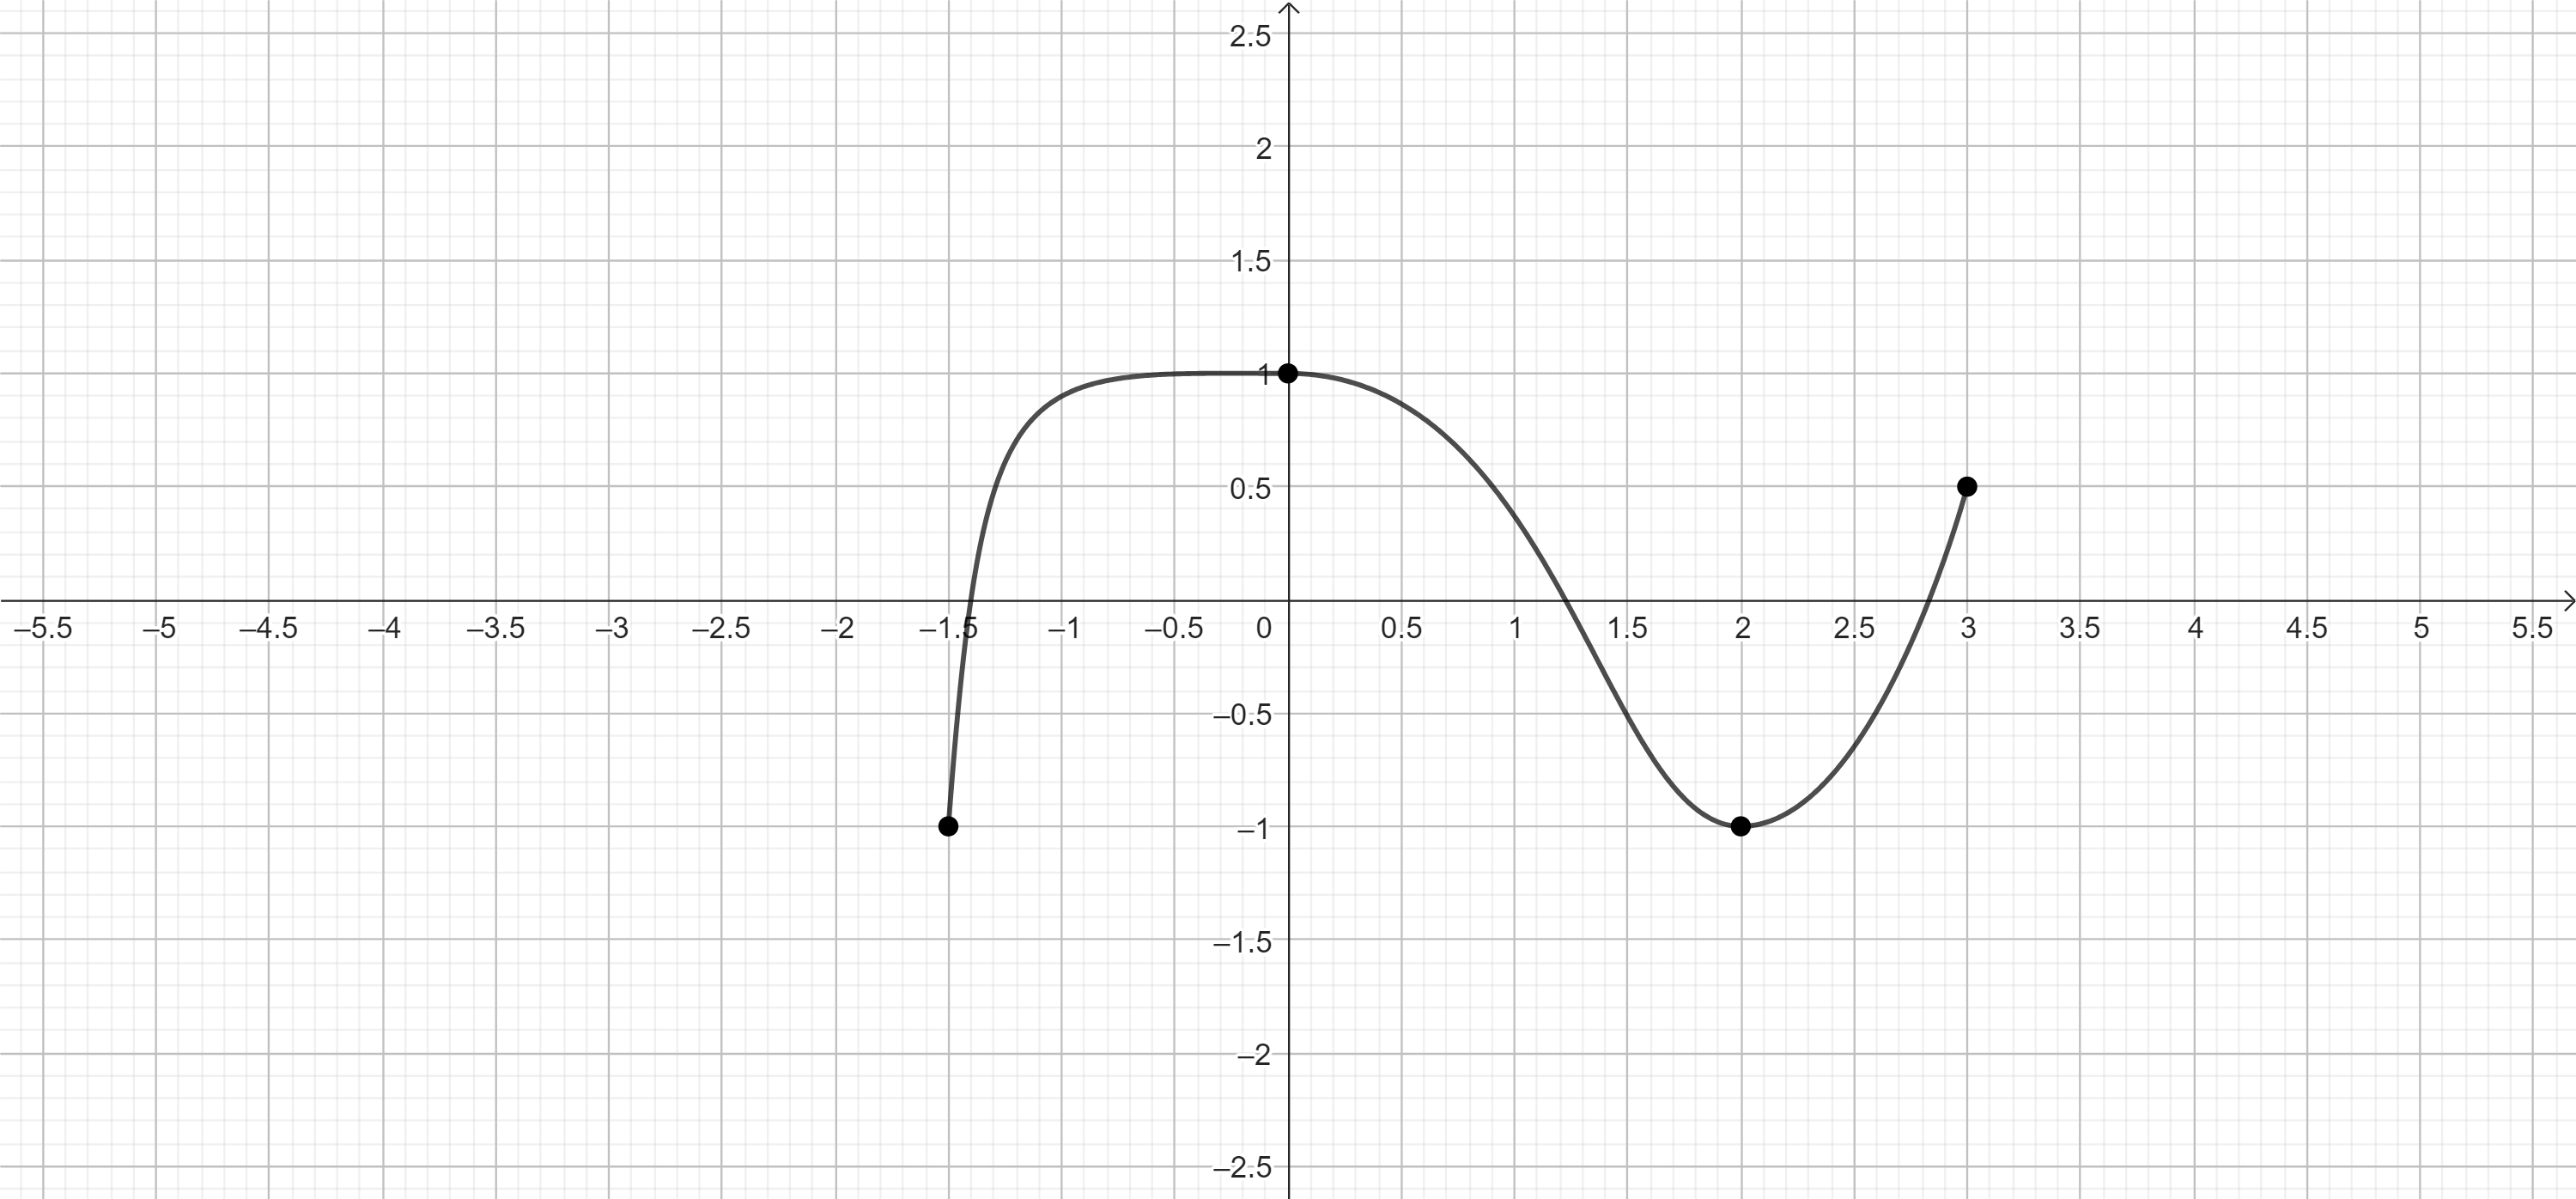
\includegraphics[scale=1.5]{Fonction2.png}
\end{center}
\end{questions}

\end{document}